\section{Countability and Separation}

    \begin{definition}[1st-Countability]
      A space $X$ is said to have a countable basis at $x$ if there exists a sequence $N_1, N_2, ...$ of open neighborhoods of $x$ such that for any neighborhood $N$ of $x$, there exists an integer $i$ such that $N_i \in N$. That is, the countable basis of neighborhoods get arbitrarily small around $x$. A space $X$ satisfying this axiom at every point $x \in X$ is said to be a \textbf{first-countable space}. 
    \end{definition}

    In particular, every metric space is first-countable, since we can construct the sequence of open balls $B (x, \frac{1}{n})$ for each $n \in \mathbb{N}$ which forms a countable basis at $x$. We now generalize some previous statements about metric spaces to statements about first-countable spaces. 

    \begin{theorem}
      Let $X$ be a space satisfying the first countability axiom, and let $A \subset X$. 
      \begin{enumerate}
        \item $x \in \bar{A}$ if and only if there exists a sequence of points in $A$ converging to $x$. 
        \item The function $f: X \longrightarrow Y$ is continuous if and only if for every convergent sequence $(x_n) \rightarrow x$ in $X$, the sequence $\big( f(x_n)\big) \rightarrow f(x)$ in $Y$. 
      \end{enumerate}
    \end{theorem}

    \begin{definition}[2nd-Countability]
      A topological space $X$ is said to satisfy the \textbf{second countability axiom} if $X$ has a countable basis for its topology.
    \end{definition}

    \begin{proposition}
      Second countability implies first countability. 
    \end{proposition}
    \begin{proof}
      If $\B$ is a countable basis for the topology of $X$, then the subset of $\B$ consisting of elements containing the point $x$ is a countable basis at $x$. 
    \end{proof}

    \begin{example}
      The real line $\mathbb{R}$ is second countable. We can contrust a countable basis as the set of all open intervals $(a, b)$ with rational end points. Likewise, $\mathbb{R}^n$ has a countable basis, which is the collection of all products of intervals having rational end points. Additionally, $\mathbb{R}^\omega$ has a countable basis. It is the collection of all products
      \begin{equation}
        \prod_{n \in \mathbb{N}} U_n
      \end{equation}
      where $U_n$ is an open interval with rational endpoints for finitely many values of $n$ and $U_n = \mathbb{R}$ for all other values of $n$. 
    \end{example}

    \begin{example}
      In the uniform topology, $\mathbb{R}^\omega$ satisfies the first countability axiom (since it is metrizable). 
    \end{example}

    \begin{theorem}
      A subspace of a first and second countable space is first and second countable, respectively. A countable product of first and second countable space is first and second countable, respectively. 
    \end{theorem}

    \begin{theorem}
      A subset $A$ of space $X$ is said to be \textbf{dense} in $X$ if $\bar{A} = X$. 
    \end{theorem}

    \begin{theorem}
      Suppose that $X$ has a countable basis. Then, 
      \begin{enumerate}
        \item Every open cover of $X$ has a countable subcover. 
        \item There exists a countable subset of $X$ which is dense in $X$. 
      \end{enumerate}
    \end{theorem}
    \begin{proof}
      Listed. 
      \begin{enumerate}
        \item Let $\B = \{B_n\}_{n \in \mathbb{N}}$ be a countable basis for $X$, and let $\mathscr{A}$ be an open covering of $X$. For each integer $n \in \mathbb{N}$, chose an element $A_n \in \mathscr{A}$ containing the basis element $B_n$. The newly formed collection $\mathscr{A}^\prime$ of all the $A_n$'s is countable since it is indexed according to a subset of $\mathbb{N}$. Furthermore, since $B_n \subset A_n$ for every $B_n$ in the basis, the $A_n$ clearly covers $X$. 

        \item From each nonempty basis element $B_n$, we choose a point $x_n$. The set 
        \begin{equation}
          D \equiv \{x_n \; | \; n \in \mathbb{N}\}
        \end{equation}
        is dense in $X$, since given any $x \in X$, every open basis element $B_x$ about $x$ intersects $D$. That is, 
        \begin{equation}
          B_x \cap D \neq \emptyset
        \end{equation}
        meaning that the set of points $x_n$ get arbitrarily close to $x$. 
      \end{enumerate}
    \end{proof}

    \begin{definition}[Lindelof Space]
      A space for which every open covering contains a countable subcovering is called a \textbf{Lindelof space}. 
    \end{definition}

    \begin{definition}[T2-Separability]
      A topological space $X$ is called a \textbf{Hausdorff space} if for each pair of distinct points $p, q \in X$, there exists neighborhoods $U_p, U_q$ that are disjoint. $X$ is also said to be \textbf{$t_2$-separable.}
      \begin{center}
        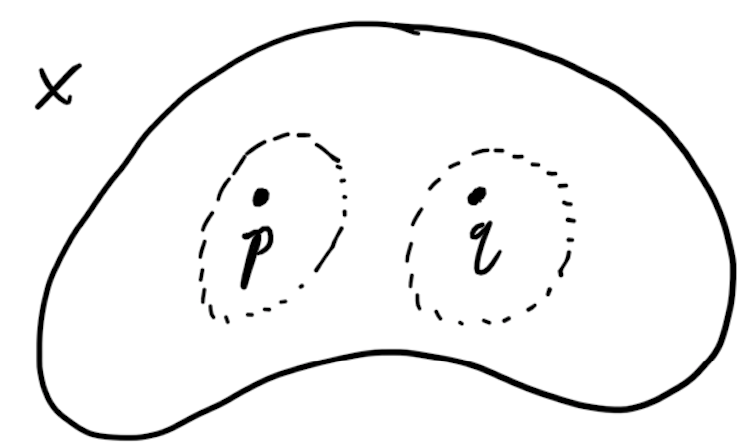
\includegraphics[scale=0.35]{img/Hausdorff_Space_Separability.PNG}
      \end{center}
    \end{definition}

    \begin{theorem}
      Every finite point set in a Hausdorff space $X$ is closed. 
    \end{theorem}
    \begin{proof}
      It suffices to show that every one point set $\{x_0\}$ is closed. If $x$ and $x_0$ are distinct points, then by definition of Hausdorff spaces they have disjoint neighborhoods $U_x$ and $U_{x_0} \implies x \not\in \bar{\{x_0\}} \implies \{x_0\} = \bar{\{x_0\}}$, so $\{x_0\}$ is closed. 
    \end{proof}

    \begin{theorem}
      Given Hausdorff space $X$ and subset $A \subset X$ a point $x$ is a limit point of $A$ if and only if every neighborhood of $x$ contains infinitely many point of $A$. 
    \end{theorem}
    \begin{proof}
      We prove both directions
      \begin{enumerate}
        \item $(\rightarrow)$ Assume that $x$ is a limit point of $A$ with some neighborhood $U_x$ intersecting $A$ in finitely many points. Then, let the points of intersections be 
        \begin{equation}
          \{x_1, ..., x_n\} = A \cap \{U_x \setminus \{x\} \}
        \end{equation}
        But $U_x \setminus \{x\}$ is open $\implies H \equiv \{U_x \setminus ( \{x\} \cup \{x_1, ..., x_n\})\}$ is open. But $H \cap A = \emptyset$, contradicting the assumption that $x$ is a limit point. 

        \item $(\leftarrow)$ Simple. 
      \end{enumerate}
    \end{proof}

    \begin{theorem}
      The product of 2 Hausdorff spaces is Hausdorff. A subspace of a Hausdorff space is a Hausdorff space. 
    \end{theorem}

    Generally, mathematicians consider the Hausdorff condition as a mild extra conditions on topological spaces that make it much easier to deal with. We will assume that most of the topological spaces we work with are Hausdorff. 

    \begin{definition}[Regular Spaces]
      Suppose that one-point sets are closed in $X$. Then, $X$ is said to be \textbf{regular} if for each pair consisting of a point $x$ and a closed set $B$ disjoint from $x$, there exist disjoint open sets containing $x$ and $B$, respectively. $X$ is also said to be $t_3$-separable. 
    \end{definition}

    \begin{definition}[Normal Spaces]
      The space $X$ is said to be \textbf{normal} if for each pair $A, B$ of disjoint closed sets of $X$, there exist disjoint open sets containing $A$ and $B$, respectively. $X$ is also said to be $t_4$-separable. 
    \end{definition}

    \begin{lemma}
      Let $X$ be a topological space. Let one-point sets in $X$ be closed. 
      \begin{enumerate}
        \item $X$ is regular if and only if given a point $x \in X$ and a neighborhood $U$ of $x$, there is a neighborhood $V$ of $x$ such that $\bar{V} \subset U$. 
        \item $X$ is normal if and only if given a closed set $A$ and an open set $U$ containing $A$, there exists an open set $V$ containing $A$ such that $\bar{V} \subset U$. 
      \end{enumerate}
    \end{lemma}

    \begin{theorem}
      \begin{enumerate}
        \item A subspace of a Hausdorff space is Hausdorff; a product of Hausdorff spaces is Hausdorff. 
        \item A subspace of a regular space is regular; a product of regular spaces is regular. 
        \item However, a subspace of a normal space is not necessarily normal; a product of normal spaces is not necessarily normal. 
      \end{enumerate}
    \end{theorem}

    \begin{theorem}
      Every metrizable space is normal. 
    \end{theorem}

    \begin{theorem}
      Every compact Hausdorff space is normal. 
    \end{theorem}

    \begin{theorem}
      Every regular space with a countable basis is normal. 
    \end{theorem}

    \begin{theorem}
      Every well-ordered set $X$ is normal in the order topology. 
    \end{theorem}

  \subsection{The Urysohn Lemma}

    \begin{theorem}[Urysohn Lemma]
      Let $X$ be a normal space, and let $A, B$ be disjoint closed subsets of $X$. Let $[a,b]$ be a closed interval in the real line. Then there exists a continuous map
      \begin{equation}
        f: X \longrightarrow [a,b]
      \end{equation}
      such that $f(x) = a$ for every $x \in A$ and $f(x) = b$ for every $x \in B$. 
    \end{theorem}

    \begin{definition}[Separation by Continuous Function]
      If $A$ and $B$ are two subsets of the topological space $X$, and if there is a continuous function $f: X \longrightarrow [0,1]$ such that $f(A) = \{0\}$ and $f(B) = \{1\}$, it is said that \textbf{$A$ and $B$ can be separated by a continuous function}. 
    \end{definition}

    More colloquially, the lemma states that if every pair of disjoint closed sets in $X$ can be separated by disjoint open sets, then each such pair can be separated by a continuous function. 

    \begin{theorem}[Tietze Extension Theorem]
      Let $X$ be a normal space and let $A$ be a closed subset of $X$. 
      \begin{enumerate}
        \item Any continuous map of $A$ into the closed interval $[a,b] \subset \mathbb{R}$ may be extended to a continuous map of all $X$ into $[a,b]$. 
        \item Any continuous map $A$ into the reals $\mathbb{R}$ may be extended to a continuous map of all of $X$ into $\mathbb{R}$. 
      \end{enumerate}
    \end{theorem}

  \subsection{The Urysohn Metrization Theorem}

    \begin{theorem}[Urysohn Metrization Theorem]
      Every regular space $X$ with a countable basis is metrizable. 
    \end{theorem}

    \begin{theorem}[Imbedding Theorem]
      Let $X$ be Hausdorff. Suppose that 
      \begin{equation}
        \{f_\alpha\}_{\alpha \in J}, \; f_\alpha: X \longrightarrow \mathbb{R}
      \end{equation}
      is a collection of continuous functions satisfying the requirement that for each point $x_0 \in X$ and each neighborhood $U$ of $x_0$, there is an index $\alpha$ such that $f_\alpha$ is positive at $x_0$ and vanishes outside $U$. Then, the function 
      \begin{equation}
        F: X \longrightarrow \mathbb{R}^J, \; F(x) \equiv \big( f_\alpha (x)\big)_{\alpha \in J}
      \end{equation}
      is an \textbf{imbedding} of $X$ in $\mathbb{R}^J$.
    \end{theorem}

